% Created 2024-06-22 Sat 16:11
% Intended LaTeX compiler: pdflatex
\documentclass[11pt]{article}
\usepackage[utf8]{inputenc}
\usepackage[T1]{fontenc}
\usepackage{graphicx}
\usepackage{longtable}
\usepackage{wrapfig}
\usepackage{rotating}
\usepackage[normalem]{ulem}
\usepackage{amsmath}
\usepackage{amssymb}
\usepackage{capt-of}
\usepackage{hyperref}
\usepackage[backend=bibtex]{biblatex}
\addbibresource{/home/laurent/Documents/code/breast-cancer-cmmd/report/refs.bib}
\usepackage{fancyvrb}
\DefineVerbatimEnvironment{verbatim}{Verbatim}{framerule=0.5mm,frame=lines,numbers=left,samepage=true}
\bibliography{refs.bib}
\author{Laurent Lejeune}
\date{\today}
\title{Breast Cancer Screening from Mammography Images\\\medskip
\large Investigating Multi-View and Multi-Task Approaches}
\hypersetup{
 pdfauthor={Laurent Lejeune},
 pdftitle={Breast Cancer Screening from Mammography Images},
 pdfkeywords={},
 pdfsubject={},
 pdfcreator={Emacs 29.3 (Org mode 9.6.24)}, 
 pdflang={English}}
\begin{document}

\maketitle
\tableofcontents


\section{Introduction}
\label{sec:orgc84fcdb}

We aim to develop a complete pipeline that predicts the malignancy of tumors contained
in mammograms using a modern supervised Machine Learning method.

In particular, we leverage an architecture based on a Convolutional Neural Network,
which we setup as a classifier.

We further pursue two axes of experimentation. The first attempts to smooth-out the inherently
noisy label set by aggregating several views of the same breast, while the second
adds an auxiliary task that explicitly leverages visual cues related to the type of abnormality.

We start by presenting the Chinese Mammography Database (CMMD), our dataset of
choice in this work, and emphasize the challenges that it brings in the setting of cancer prediction.

Next, in the Methods section, we formulate our problems,
namely how we combine the different classification tasks, and how
we merge multiple view-angles of the same breast-sample,
and describe our architecture and training strategy.

In the Results section, we provide quantitative figures to compare the performance of our
different configurations with the state-of-the-art.

Last, we conclude by giving an outlook and suggest possible improvements.

\section{The Chinese Mammography Database (CMMD)}
\label{sec:orgf677314}

\subsection{\label{screening}Screening}
\label{sec:orgf0e00ca}

We use the publicly available Chinese Mammography Database (CMMD) \autocite{cai23},
which originally contains \(\approx 1871\) patients screened for breast cancer.
These are then filtered-out so as to match the following criteria:

\begin{itemize}
\item Patients with history of previous breast biopsy within 1 week, or any therapy for breast lesions
prior to mammography.
\item Patients with breasts prosthesis.
\item Images with substantial motion artifact.
\end{itemize}

This reduces the number of patients to \(1775\).

\subsection{Annotations}
\label{sec:orgc3b642f}

Each \emph{breast} is analyzed by domain experts so as to assign the following
target variables:

\begin{itemize}
\item \(y_{t} \in \{\text{benign}, \text{malignant}, \text{none}\}\) indicates the type of tumor.
\item \(y_{a} \in \{\text{calcification}, \text{mass}, \text{both}\}\) indicates the type of abnormality, where \texttt{both} means that both \texttt{calcification} and \texttt{mass} are present.
\item \(y_s \in \{\text{luminal-A}, \text{luminal-B},\text{HER2-positive},\text{triple-negative},\text{missing}\}\) a
subtype information (possibly missing).
\end{itemize}

\subsection{\label{limitations}Limitations}
\label{sec:org97ca8d8}

The CMMD dataset is challenging to use in a Machine Learning setting.
Indeed, for a ML practitioner, coherent labels are crucial to fully exploit
modern techniques. In particular, we found that this dataset includes
the following sources of noise:

\begin{enumerate}
\item Each study contains 2 views per breast. This is due to the fact that the visual cues
that are relevant to distinguish a benign from a malignant tumor are
 sometimes absent from one of the two available views, thereby justifying redundancy.
 In other words, the labels that directly refer to visual cues, i.e. \(y_{a}\),
 have been associated with two views (images), while one of the two could contain no
 such cue.

\item While the abnormality labels \(y_{a}\) seem to refer to well-defined visible objects,
we find that these come in at least 2 forms: compact blobs, and clusters.
Importantly, the latter distinction of form is a crucial clue
to identify malignancy \autocite{azam21}.
Again, this adds another component of noise in our label set.

\item In our best understanding, \(y_{t}\), the malignant/benign label, has been
assigned following a thorough histopathological protocol, and not solely on the
basis of the imaging protocol.
\end{enumerate}

While there exists many techniques to deal with noisy labels \autocite{song22},
we choose to investigate on simple arithmetic operations as part of the
training phase.

\subsection{Exploration}
\label{sec:orgb971ab3}

We show the distribution of abnormalities with respect to tumor type on Fig. \ref{fig:distributions},
and show example images on Fig. \ref{fig:preview}.

\begin{figure}[htbp]
\centering
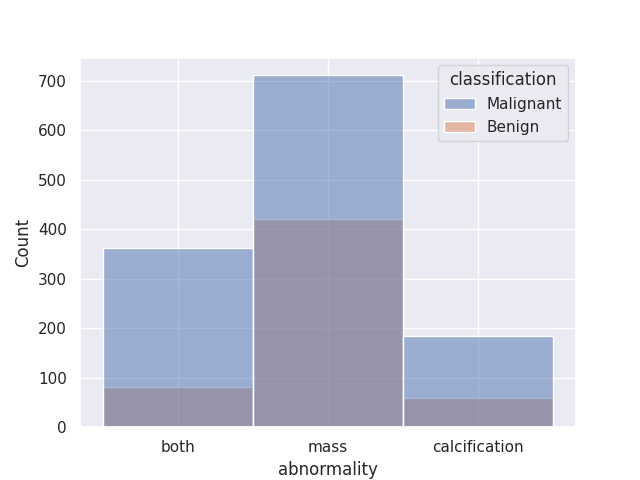
\includegraphics[width=.9\linewidth]{./images/distrib.png}
\caption{\label{fig:distributions}Distributions of abnormalities for diagnosis}
\end{figure}

\begin{figure}[htbp]
\centering
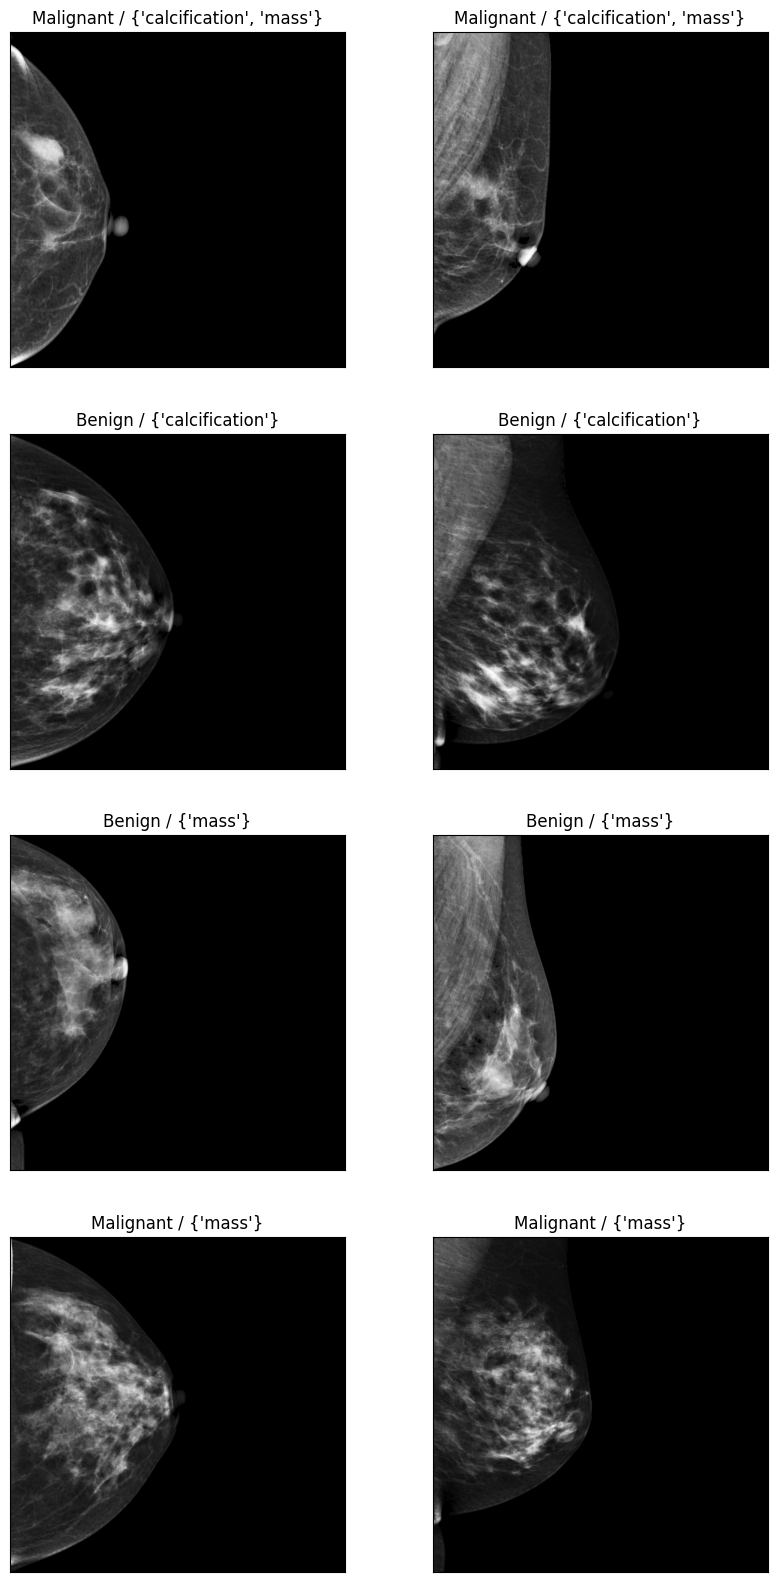
\includegraphics[width=9cm]{./images/previews.png}
\caption{\label{fig:preview}Example images. On each row, we show two views of the same breast.}
\end{figure}

\subsection{\label{split}Curation and Splitting}
\label{sec:org06b08c7}

As we endeavour to use the CMMD dataset to produce an ML solution, we
perform a curation step and split all images in a train, validation, and testing splits.

In addition to the filtering criteria described in Sec. \ref{screening}, we further
discard images that have identical hashes following the authors's recommendations \footnote{\url{https://www.cancerimagingarchive.net/collection/cmmd/}}.

In our best understanding, there does not exists an official and publicly avaible train/val/test
split. We therefore make our own through the following steps:

\begin{enumerate}
\item We discard all images that have no labels \(y_t\) and \(y_a\).
\item We group all images by breast, i.e. each group contain two views of the same breast.
\item To perform cross-validation, we divide all groups using a stratified
shuffled splitting strategy, where each split
must contain the same proportion of \(y_t\) and \(y_a\). Our splits contain \(60\), \(20\),
 and \(20\%\) of images for the train, validation, and testing set, respectively.
\end{enumerate}

\section{Methods}
\label{sec:org922a1f7}

We aim to learn a predictor that determines whether a given mammography study
contains a malignant or benign tumor.

At its core, our model extracts features using a Convolutional Neural Network,
and follows with two parallel classification heads.

We now develop our composite objectives and multi-view classification approaches.

\subsection{\label{multiview}Learning with Multiple Views}
\label{sec:org0604f7c}

Following previous works in breast cancer screening,
we implement and test several ways to handle the fact that
labels are assigned to studies, and not individual images.

This problem setting is referred to as ``Multi-View''.
In particular, we implement:

\begin{enumerate}
\item \textbf{Averaging of output probabilities}:  We forward-pass all images of the same study
and compute the mean probability output prior to computing the loss and applying
back-propagation.
\item \textbf{Averaging of features}: Following \autocite{geras17} \autocite{seeland21}, we first compute the mean feature vector of all images of the same
study. We then pass this vector into the classification layer and proceed as in
previous approach.
\item \textbf{Max aggregation of features}: Similar to previous approach, but we compute the max descriptors instead.
\item \textbf{Feature concatenation}: Following \autocite{wu19} \autocite{chen22}, we concatenate feature
vectors and proceed as in previous approaches.
\end{enumerate}

\subsection{Auxiliary Task}
\label{sec:org4a75870}

We investigate the relevance of multi-task learning (MTL) in breast cancer screening,
While authors in \autocite{tardy22} demonstrate the benefits of MTL
by augmenting the main objective with
4 other auxiliary tasks, namely that of predicting the view-angle and
regressing on the breast density,
we choose to add the auxiliary task of identifying abnormalities.

Although breast density is another useful indicator, we do not have this information for the CMMD dataset. The challenge of this auxiliary tasks lies in the fact, that unlike image laterality or breast density, the abnormality type is less obvious in the mammography image, and also, as mentioned above, some views may not contain it at all.

Furthermore, we learn from \autocite{azam21} that overall, pathological and sane
cases show different \emph{forms} of calcification, i.e. malignant cases show smaller and clustered
microcalcifications, while benign cases tend to create large blobs.

Without justification, and for the sake of experimentation,
we extrapolate the above result to the \emph{mass} abnormality, and assume
that it also comes in specific shape/form depending on the benign/malignant
scenario.

Formally, we add for each abnormality-type \emph{calcification} and \emph{mass},
a parallel classification head to our backbone, that are trained using
3 labels each: \textbf{benign-form}, \textbf{malignant-form}, and \textbf{absent}.
These artificial labels are trivially derived from the tumor-classification and
the abnormality label provided by domain experts.
The studies containing both type of abnormalities are excluded from this, due to the added noise that would be introduced since we cannot, without the help of an expert, know which abnormality type is responsible for the label.

In these branches, we implement and investigate similar aggregation strategies
given in Sec. \ref{multiview}.

\subsection{Architecture}
\label{sec:org53b1c82}

Our model is a Convolution Neural Network based on the ResNet34
architecture \autocite{he15}, which encodes each image into a \(512\) -dimensional feature
vector.
Next, features are mapped to probability distributions following Multi-Layer Perceptrons
and sigmoid/softmax activation functions.
We give an illustration of our model in Fig. \ref{fig:model}.

\begin{figure}[htbp]
\centering
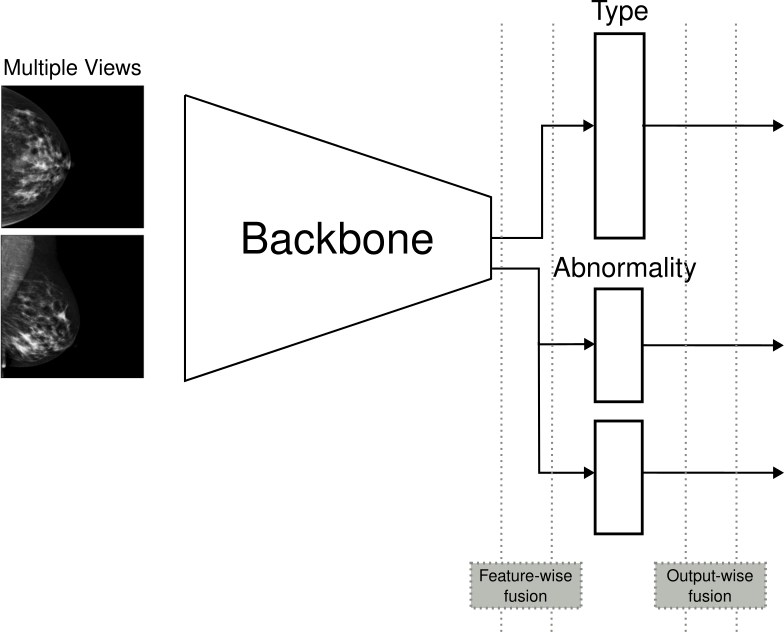
\includegraphics[width=.9\linewidth]{./images/model.png}
\caption{\label{fig:model}Our model takes as input a set of images that show several views of the same breast. We investigate on several fusion strategies (dashed columns): (1) Fuse features at bottleneck, or (2) fuse prediction outputs. We also set an auxiliary multi-label classification objective on abnormalities (bottom branch).}
\end{figure}

\subsection{Preprocessing, Training, and Validation}
\label{sec:orgb83bb30}

We convert the original images given as DICOM series into 8-bit images,
and rescale these from \(1914 \times 2294\) to \(1024 \times 1024\) pixels. We found that this
is a good compromise as it conserves most fine-grained details while
reducing computational burden.

Next, we apply a simple pre-processing pipeline inspired by \autocite{walsh22}.
In particular, we apply the non-parametric triangle thresholding operator \autocite{zack77}
to remove background noise.
Last, we apply vertical mirroring to right breasts so as to align them with left breasts.

We construct mini-batches so as to include all views of a given breast, thereby
giving \(V \times B\) images per batch, where \(V\) is the number of views,
and \(B\) is the number of breasts per-batch.

Both training objectives are weighed and summed to produce
the total loss \(\mathcal{L}\):

\begin{equation}
\mathcal{L} = \lambda_{t}\mathcal{L}_{t} + \lambda_{a}\mathcal{L}_{a}
\end{equation}

Where \(\mathcal{L}_t\) and \(\mathcal{L}_a\) optimize for tumor type
and abnormality, respectively.

After manual tuning, we set \(\lambda_t=1\) for all experiments,
and \(\lambda_a \in \{0; 0.3\}\) depending on experimental setting.

We train both our backbone and classification heads in an end-to-end manner through
gradient descent using a cross-validation strategy.
We leverage the training/validation splits described in Sec. \ref{split}, and train for
\(20\) epochs, where each epoch contains \(50\) randomly sampled mini-batches,
where each mini-batch contains \(16\) images, i.e. \(8\) breasts.

Our gradients are computed using the Adam optimizer with a learning rate of
\(5 \times 10^{-5}\).

For fair comparison with the state-of-the-art \autocite{walsh22}, we select the model so
as to maximize the area under the ROC curve on the validation set.

\section{Results}
\label{sec:org6437d66}

We compute performances on the benign/malignant classification task
on the testing dataset for each of the following named configurations:

\begin{itemize}
\item \texttt{mean-feats}: Mean aggregation of features
\item \texttt{max-feats}: Max aggregation of features
\item \texttt{concat-feats}: Concatenation of features
\item \texttt{output}: Mean probability output
\end{itemize}

Our results are sorted according to AUC(ROC) metric.
We also provide the average precision (\texttt{AP}), i.e. the area under the PR-RC curve.

Another experimental parameter, \texttt{with aux task}, takes value \texttt{True} when we jointly optimize for the
auxiliary task that classifies abnormalities.

\begin{verbatim}
 fusion mode  with aux. task  AUC(ROC)    AP
  mean-feats            True     0.679 0.830
  mean-feats           False     0.669 0.825
      output            True     0.656 0.801
      output           False     0.597 0.776
   max-feats            True     0.580 0.755
   max-feats           False     0.566 0.745
concat-feats            True     0.494 0.720
concat-feats           False     0.410 0.662
\end{verbatim}


Interestingly, the \texttt{concat-feats} mode performs very poorly.
We hypothesize that this might be due to the fact
that we do not take into account the view-angle into account when
concatenating.

\section{Discussion, Conclusion and Future Works}
\label{sec:orgd8abe55}

We contributed a method to discriminate X-ray image sets of breasts into malignant and benign
categories.

Given that the proposed task is known to be hard, and further made more difficult by
the fact that the CMMD dataset has noisy and inconsistent labels,
we proposed techniques to smooth-out these inconsistency by leveraging multi-view and
auxiliary task objectives.

We showed that the two latter upgrades bring promising improvements.
However, we wish to emphasize that the attained performance-level remain low.
Importantly, our best model reaches performance-levels that lie substantially
below the state-of-the-art \autocite{tardy22}, while being technically more involved.
This might be due to differences in data curation, and/or splitting strategies.

Also, we believe that the proposed auxiliary task could bring much stronger
improvement, provided that abnormalities are labelled according to their actual
visual appearance. Another upgrade in these annotations could come in the form
of localization, such as bounding-boxes or delineations, as already investigated by \autocite{tang19}.



\printbibliography
\end{document}
